\documentclass[12pt,a4paper,oneside]{article}

\usepackage[utf8]{inputenc}
\usepackage[greek,english]{babel}
\usepackage{alphabeta} 

\usepackage[pdftex]{graphicx}
\usepackage[top=1in, bottom=1in, left=1in, right=1in]{geometry}
\usepackage{hyperref}
\linespread{1.06}
\setlength{\parskip}{8pt plus2pt minus2pt}
\usepackage{fancyhdr}
\widowpenalty 10000
\clubpenalty 10000
\usepackage{caption}

\usepackage{graphicx}
\newcommand{\eat}[1]{}
\newcommand{\HRule}{\rule{\linewidth}{0.5mm}}

\usepackage[official]{eurosym}
\usepackage{enumitem}
\setlist{nolistsep,noitemsep}
\usepackage[hidelinks]{hyperref}
 \usepackage[table]{xcolor}

\setlength{\parindent}{10ex}

\usepackage{lipsum}
\hypersetup{
    colorlinks=true,
    linkcolor=black,
    filecolor=magenta,      
    urlcolor=blue,
}

\begin{document}

\renewcommand{\contentsname}{Περιεχόμενα}

\renewcommand{\refname}{Αναφορές}

%===========================================================
\begin{titlepage}
\begin{center}

% Top 
\includegraphics[width=0.55\textwidth]{upatras_logo.jpg}~\\[2cm]


% Title
\HRule \\[0.4cm]
{ \LARGE 
  \textbf{PROJECT TΕΧΝΟΛΟΓΙΑ ΛΟΓΙΣΜΙΚΟΥ}\\[0.4cm]
  \emph{Project-description-v0.1}\\[0.4cm]
}
\HRule \\[1.5cm]



% Author
{ \large
  \includegraphics[width=0.5\textwidth]{logo.png}~\\[2cm]
 
}

\vfill

\textsc{\large Τμήμα Μηχανικών Ηλεκτρονικών Υπολογιστών \& Πληροφορικής}\\[0.4cm]


% Bottom
{\large \selectlanguage{greek}\today}
 
\end{center}
\end{titlepage}
\pagestyle{fancy}
\fancyhead[RO,LE]{Project-description-v0.1}
\fancyhead[LO,CE]{\includegraphics[width=0.05\textwidth]{logo.png}}
\centering
Ακολουθεί ο πίνακας με τα ονόματα και τα ΑΜ της ομαδάς μας:

\centering
\begin{tabular}{ |p{4cm}|p{4cm}|p{3cm}|}
\arrayrulecolor{gray}
 \hline
 \multicolumn{3}{|c|}{Μέλη} \\
 \hline
 ΕΠΩΝΥΜΟ& ΟΝΟΜΑ & Α.M\\
 \hline
 ΛΙΟΥΜΗΣ   & ΕΥΑΓΓΕΛΟΣ    & 1054325\\
 ΣΧΙΖΑΣ &  ΝΙΚΟΛΑΟΣ & 1054394\\
 ΛΥΡΟΥ & ΔΗΜΗΤΡΑ & 1057774\\
 ΜΠΟΥΡΣΑΛΗΣ   & ΕΜΜΑΝΟΥΗΛ & 1056284\\
\hline 

\end{tabular}


\vspace{7cm}
\raggedright
\textbf{Editors:}
\newline
Νίκος Σχίζας
\newline
Δήμητρα Λύρου
\newline
Ευάγγελος Λιούμης
\newline
Εμμανουήλ Μπούρσαλης


\vspace{7cm}

\raggedright
\textbf{Εργαλεία:}

    Overleaf
    
    Microsoft Word

    Adobe XD
\newpage

%===========================================================

\tableofcontents
\addtocontents{toc}{\protect\thispagestyle{empty}}

\newpage
\setcounter{page}{1}

%===========================================================
%===========================================================

\section{Περιγραφή Έργου}\label{sec:intro}
\pagestyle{fancy}
\fancyhead[RO,LE]{Project-description-v0.1}
\fancyhead[LO,CE]{\includegraphics[width=0.05\textwidth]{logo.png}}

\hspace{1cm} Η \textbf{Ν.Ο.Ε.(Νοσοκομειακή Οργάνωση Ελλάδος)} πρόκειται για μια σύγχρονη νοσοκομειακή βάση δεδομένων στην οποία θα γίνεται η καταχώρηση και η διαχείριση όλων των νοσοκομείων, των ιατρών και των ασθενών τους, καθώς και κάποιων τμημάτων τους. Στο σύστημα αυτό, θα έχουν πρόσβαση το νοσοκομειακό προσωπικό, οι ασθενείς και το Υπουργείο Υγείας. Το προσωπικό θα εισάγεται στο σύστημα κατά την εγκατάσταση του στο εκάστοτε νοσοκομείο. Κάναμε την εξής υπόθεση εργασίας: το συγκεκριμένο project δημοπρατήθηκε από το Υπουργείο Υγείας και μέσω ανοιχτού διαγωνισμού καταφέραμε να το αναλάβουμε.   \par
\hspace{1cm}Ο \textbf{ασθενής} θα μπορεί να πραγματοποιεί την εγγραφή του στο σύστημα όποτε αυτός θελήσει εξ αποστάσεως ή υποχρεωτικά κατά την εισαγωγή του στο εκάστοτε νοσοκομείο. Η υποχρεωτική εγγραφή θα γίνεται από τη γραμματεία του νοσοκομείου, απαιτείται για τη λειτουργία του συστήματος και θα αναλυθεί παρακάτω. Η χρήση του συστήματος από τον ασθενή δεν είναι υποχρεωτική προφανώς. Κατά την εγγραφή του θα χρειαστεί να καταχωρήσει το όνομα του, το επώνυμο του, το όνομα πατρός του, τον αριθμός ταυτότητας του, το ΑΦΜ του, το ΑΜΚΑ του,  το τηλέφωνο του και το email του. Επιπλέον, θα αποθηκεύεται ένα σύντομο ιατρικό ιστορικό του για την διευκόλυνση του θεράποντα γιατρού. Σε περίπτωση που νοσηλεύεται κάπου, θα  αποθηκεύεται ο λόγος εισαγωγής του, η ημερομηνία εισαγωγής του,  ο υπεύθυνος γιατρός του, το εισιτήριο και το εξιτήριο του όταν ολοκληρωθεί η νοσηλεία.  Θα μπορεί επίσης μέσω του συστήματος να κλείσει ραντεβού με κάποιον ιατρό της επιλογής του βλέποντας τις διαθέσιμες ώρες του. Όταν το ραντεβού καταχωρηθεί με επιτυχία, ο ίδιος καθώς και ο ιατρός θα ενημερώνονται με μήνυμα ηλεκτρονικού ταχυδρομείου για τις πληροφορίες και τις ώρες του ραντεβού. Θα μπορεί επιπλέον, να αξιολογεί και να σχολιάζει προεραιτικά τον κάθε θεράποντα ιατρό του με μια κλίμακα εντός του συστήματος η οποία κυμαίνεται απο το 1 μέχρι το 5. Τέλος, θα μπορεί να βλέπει και να εξοφλεί τις  οφειλές του αν τυχόν υπάρχουν. \par
\hspace{1cm}Η \textbf{γραμματεία} του νοσοκομείου θα μπορεί μέσω του συστήματος να υπολογίζει αυτόματα το συνολικό κόστος νοσηλείας ενός ασθενή λαμβάνοντας υπόψιν την ύπαρξη ασφάλισης ή όχι. Θα μπορεί επίσης να πραγματοποιεί την εγγραφή των ασθενών στο σύστημα αν δεν υπάρχουν ήδη, διασφαλίζοντας έτσι την ομαλή λειτουργία του συστήματος και εξυπηρετώντας με αυτόν τον τρόπο τις εκαστότε λειτουργίες που παρέχονται μέσω αυτού. Τέλος, θα μπορεί να διαχειρίζεται τα εισιτήρια και τα εξιτήρια των ασθενών, τα οποία έχουμε σκοπό να είναι σε ψηφιακή μορφή. \par
\hspace{1cm}O \textbf{διευθυντής} του νοσοκομείου θα μπορεί να υπολογίζει τον ετήσιο προϋπολογισμό του νοσοκομείου και έπειτα να τον αποστέλλει στο Υπουργείο Υγείας. Θα μπορεί επίσης να βλέπει στατιστικά μέσω του συστήματος για το νοσοκομείο του και να τα αποστέλλει στο Υπουργείο για ενημέρωση. Τα στατιστικά θα περιλαμβάνουν διαθέσιμες κλίνες ανά ημέρα, ασθένειες που έχουν παρουσιαστεί, θάνατοι ανά ημέρα, εισαγωγές ανά ημέρα, μέσος όρος κόστους και μέση διάρκειας νοσηλείας. \par
\hspace{1cm}To \textbf{Υπουργείο Υγείας} θα λαμβάνει στατιστικά και προϋπολογισμούς από κάθε νοσοκομείο, θα έχει εποπτικό ρόλο και θα επεμβαίνει όποτε κρίνεται αναγκαίο. Για την ώρα δεν προβλέπεται να έχει κάποια άμεση ανάμειξη στη λειτουργία του συστήματος. \par
\newpage
\hspace{1cm}Ο \textbf{ιατρός} θα μπορεί να θέτει τις ώρες και ημέρες για τις οποίες είναι διαθέσιμος για ραντεβού. Το πρόγραμμα του θα μεταβάλλεται δυναμικά με το κλείσιμο ραντεβού από τους ασθενείς αλλά θα μπορεί να το μεταβάλλει και ο ίδιος. Επίσης, θα μπορεί να βλέπει τις αξιολογήσεις που έχει λάβει από ασθενείς. Επιπλέον,  ο ίδιος θα μπορεί να επεξεργάζεται το ιατρικό ιστορικό των ασθενών του καθώς και να έχει πρόσβαση σε πληροφορίες που έχουν να κάνουν με τους ασθενείς του. \par
\hspace{1cm}To \textbf{τμήμα προμηθείων} θα μπορεί να ετοιμάζει παραγγελίες προμηθειών με βάση τη διαθέσιμη ποσότητα της κάθε μίας. Αυτή η διαδικασία θα γίνεται αυτόματα σε καθορισμένα χρονικά διαστήματα από το σύστημα και πριν από κάθε παραγγελία και λόγω της σοβαρότητας αυτής της λειτουργίας θα απαιτείται έγκριση από τον υπεύθυνο. Για να διατηρείται κάθε στιγμή η διαθέσιμη ποσότητα των προμηθειών, θα υπάρχει μία λειτουργία στην οποία κάθε προμήθεια που παραλαμβάνεται ή καταναλώνεται θα καταχωρείται στο σύστημα. Ο υπεύθυνος θα μπορεί να κάνει χειροκίνητα παραγγελίες σε περίπτωση που κρίνει ότι υπάρχει άμεση ανάγκη. Ο χρόνος του κάθε ελέγχου για ελλείψεις θα επιλέγεται από τον υπεύθυνο με βάση την εμπειρία του στο συγκεκριμένο πόστο. \par
\hspace{1cm} \textbf{Σημαντικές διευκρινίσεις:}\par

\hspace{1cm} Για τους εργαζόμενους, εκτός από την προηγούμενη ανάλυση,θα  αποθηκεύονται για κάθε έναν: η ειδικότητα (εφόσον υπάρχει) του, το τμήμα του, η θέση εργασίας του, το νοσοκομείο στο οποίο εργάζεται καθώς και ο μισθός του σε μηνιαία βάση. 

\hspace{1cm} Για το νοσοκομείο θα καταχωρείται: η διεύθυνση του, η λίστα των εργαζομένων του, η λίστα με τα τμήματα του, οι διευθυντές του, ο αριθμός των διαθέσιμων δωματίων και θέσεων του για ασθενείς. 


\newpage

\section{Eνδεικτικές mock-up screens}\label{sec:lit-rev}
 Παραθέτουμε για την ώρα κάποια ενδεικτικά mock-up screens μέσω του εργαλείου Adobe XD ώστε να δώσουμε μια πρόχειρη ιδέα της εμφάνισης της εφαρμογής μας. Προφανώς θα υπάρξουν διαφορές με τις τελικές οθόνες καθώς και σε επόμενα παραδοτέα θα προσθεθούν περισσότερες οθόνες και βελτιωμένες σε κάποια σημεία ώστε να φανεί η εξέλιξη του έργου μας.
\newline

\begin{figure}[h!]
\centering

\includegraphics[width=1.\textwidth]{Οθόνη σύνδεσης.pdf}
\captionsetup{labelformat=empty}
\caption{Οθόνη 1: Οθόνη σύνδεσης}
\end{figure}


\begin{figure}[h!]
\centering
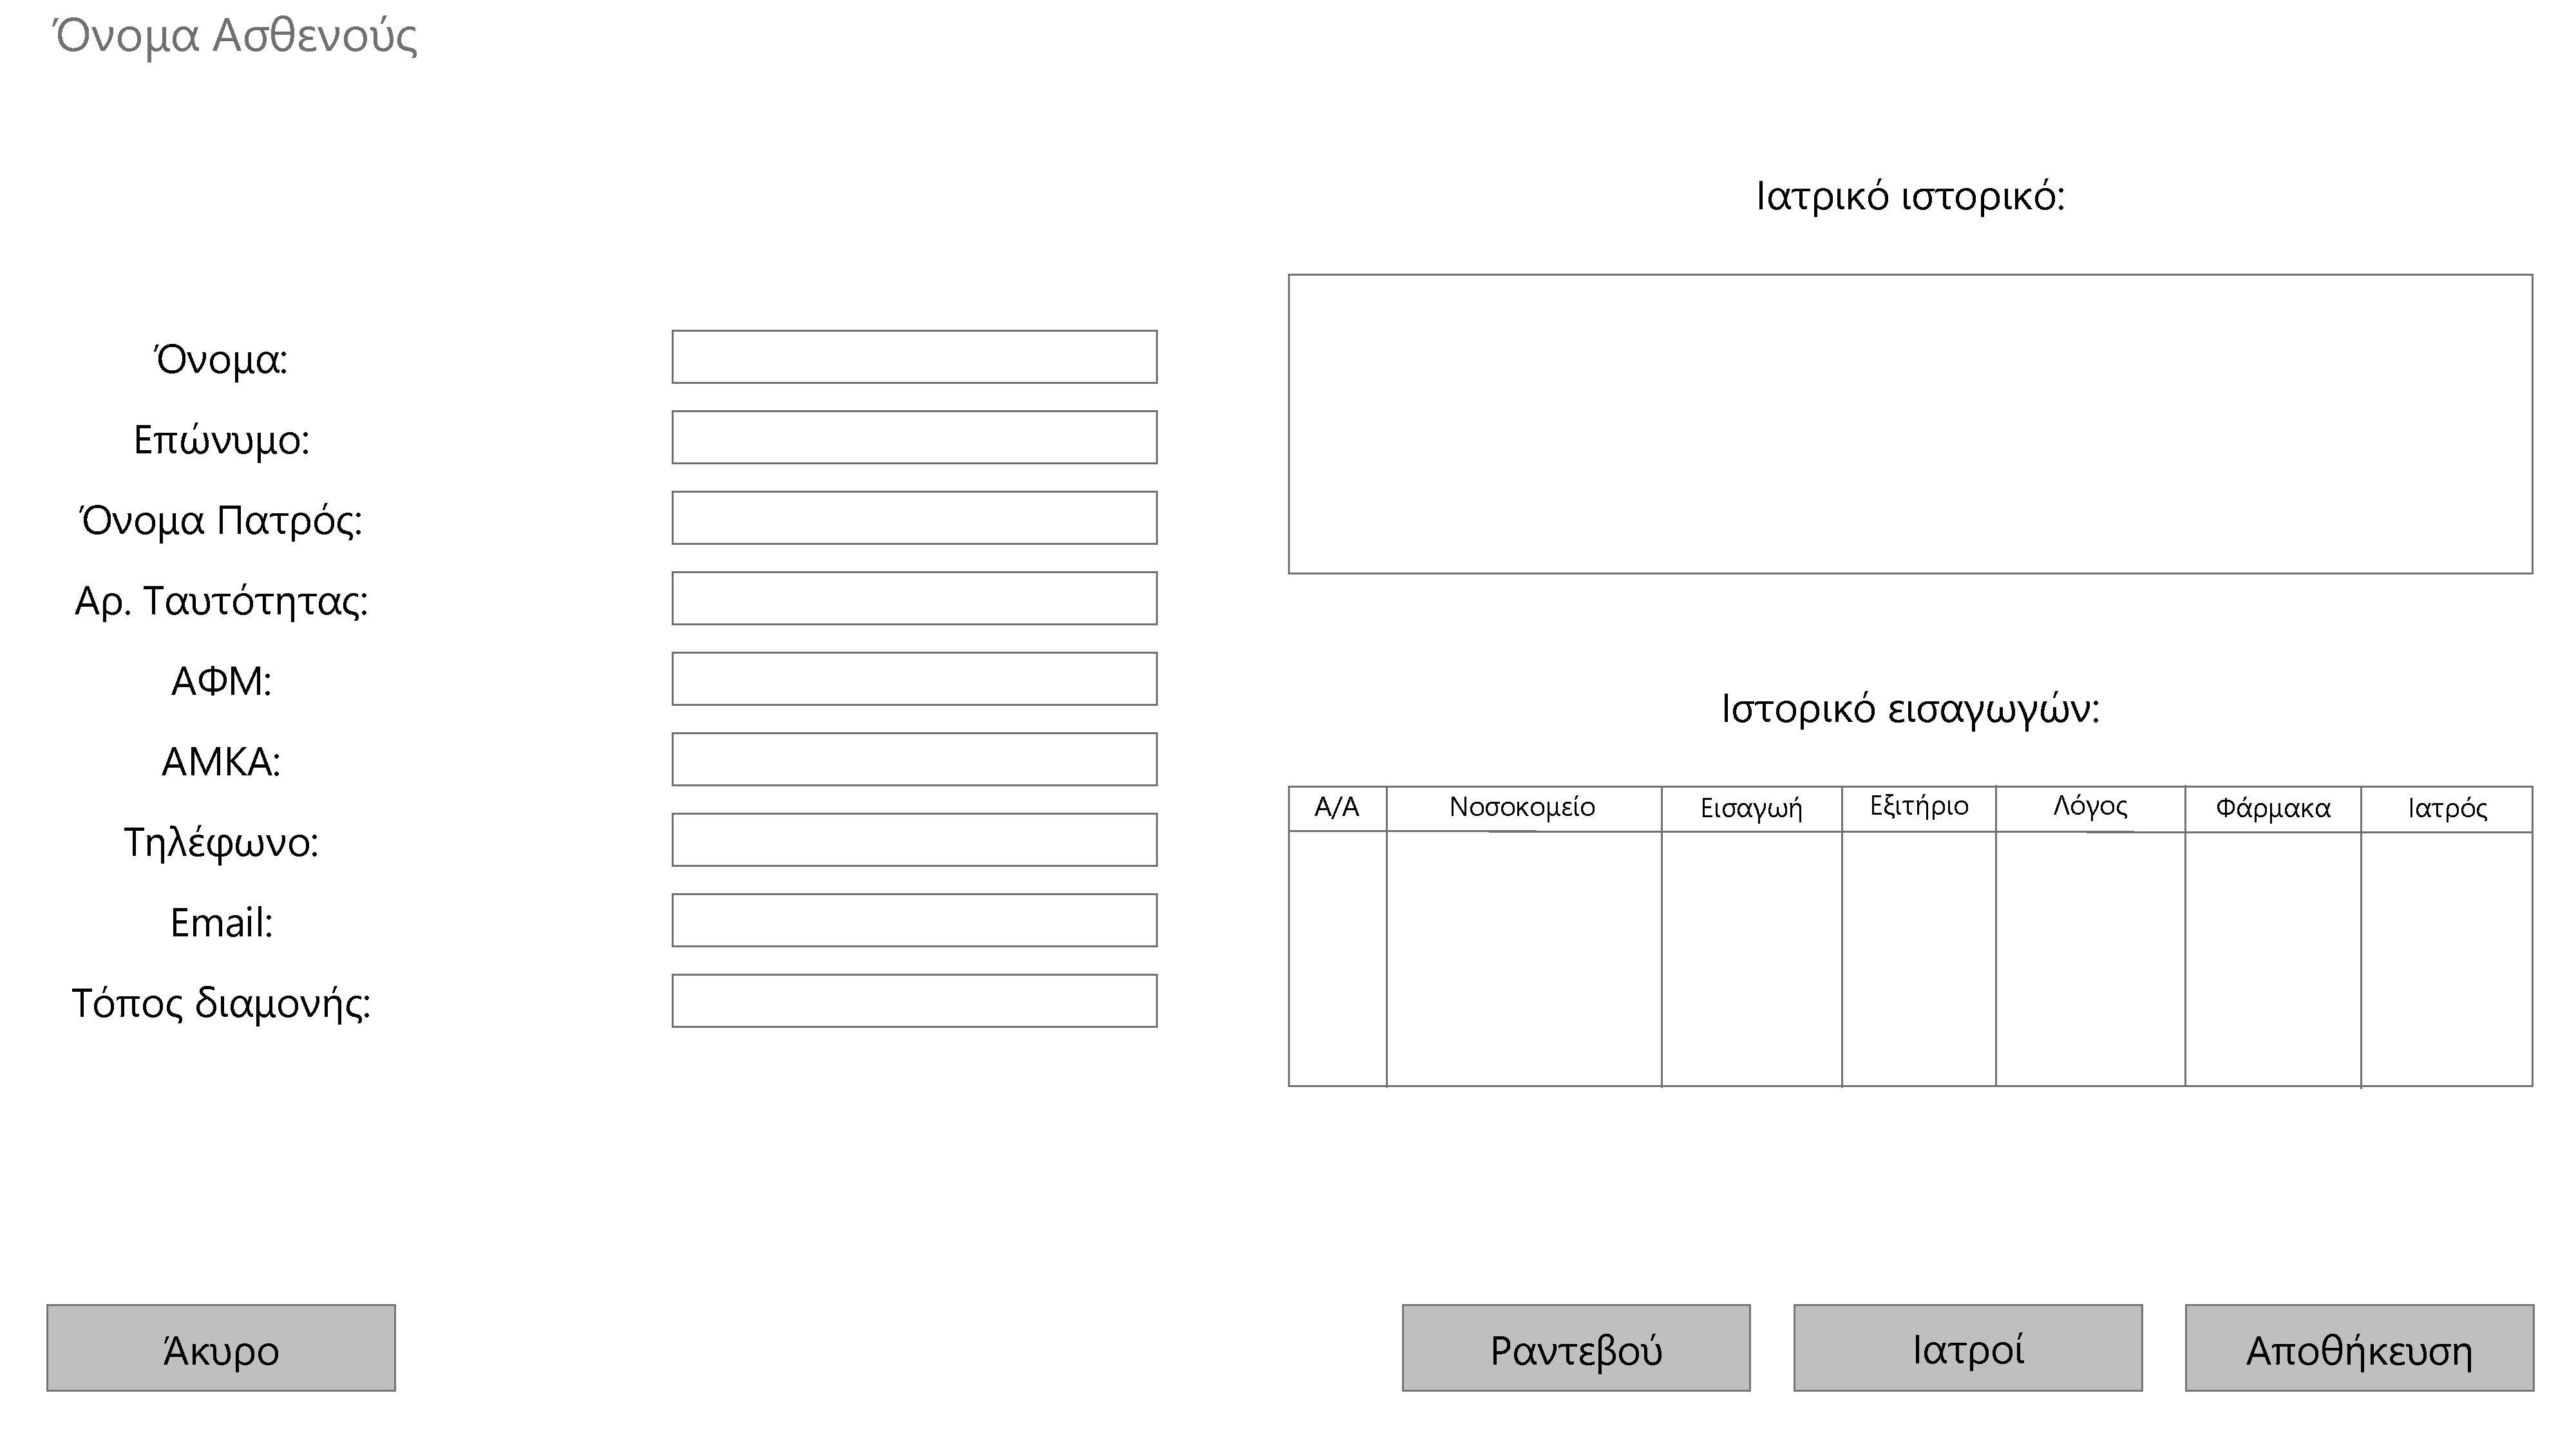
\includegraphics[width=0.9\textwidth]{Ασθενής Αρχική οθόνη.pdf}
\captionsetup{labelformat=empty}
\caption{Οθόνη 2: Ασθενής Αρχική οθόνη}
\end{figure}

\newpage
\begin{figure}[h!]
\centering
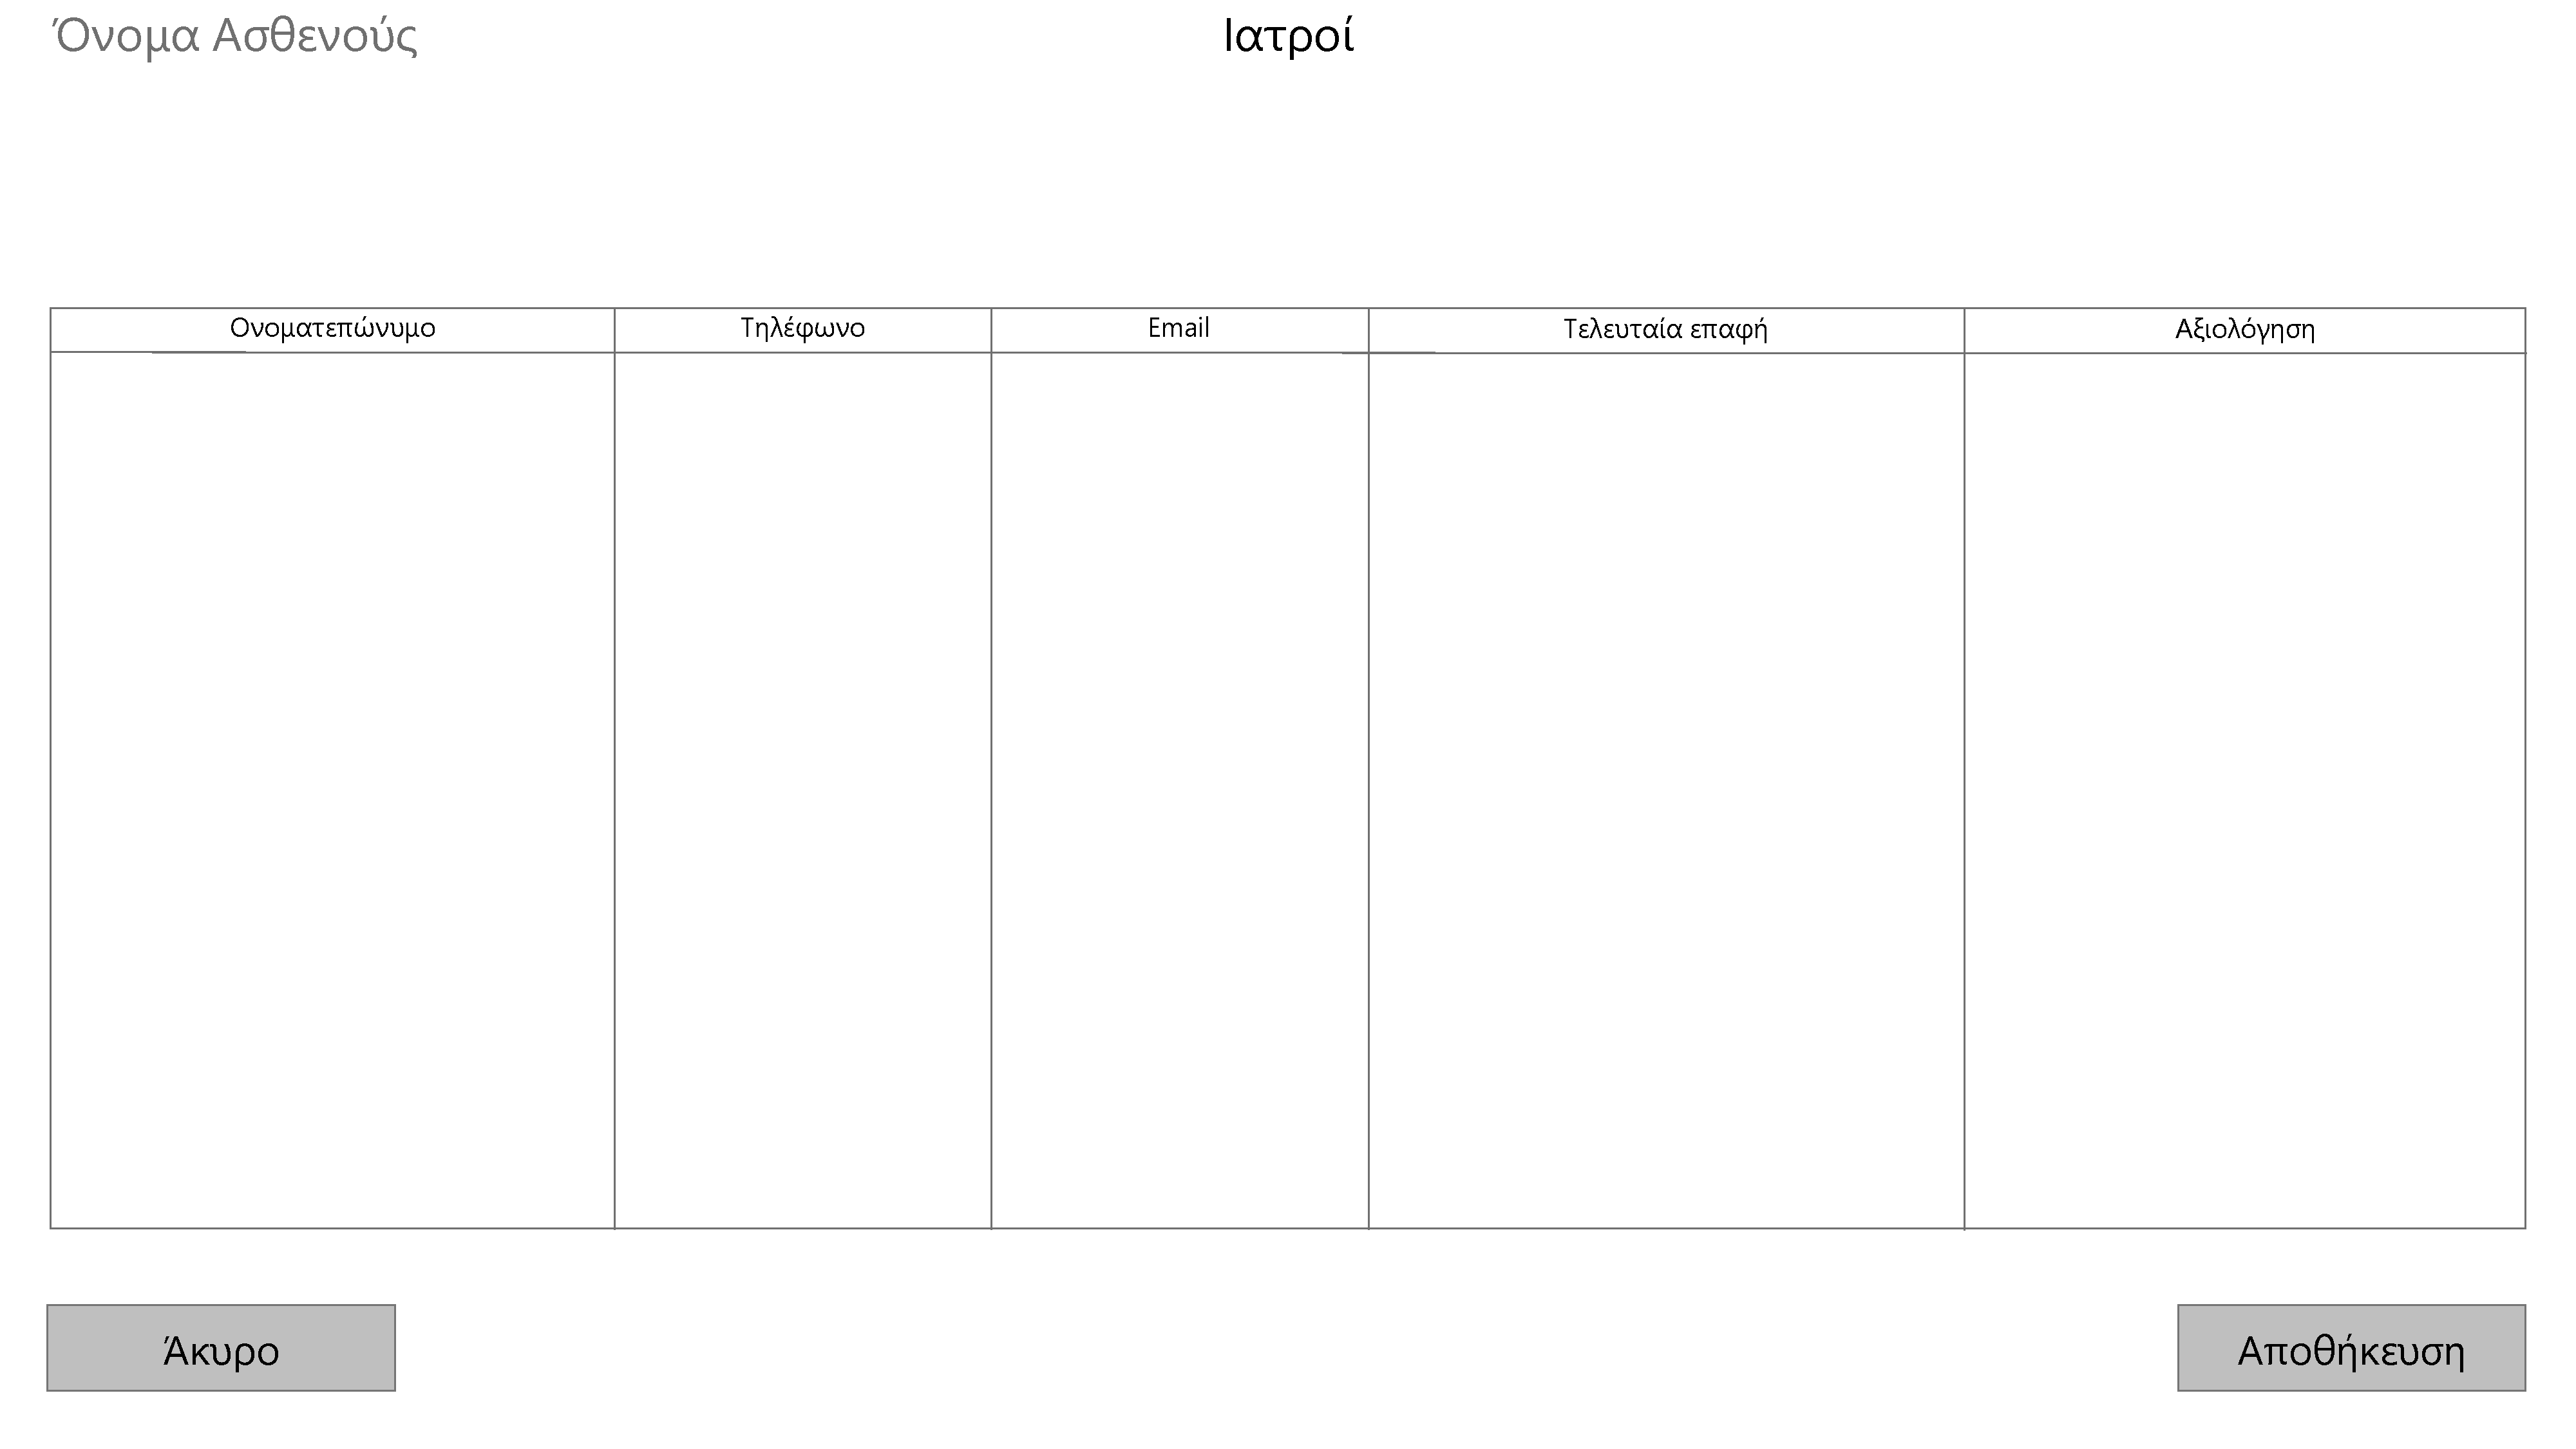
\includegraphics[width=1.1\textwidth]{Ασθενής Ιατροί.pdf}
\captionsetup{labelformat=empty}
\caption{Οθόνη 3: Ασθενής Ιατροί}
\end{figure}

\begin{figure}[h!]
\centering
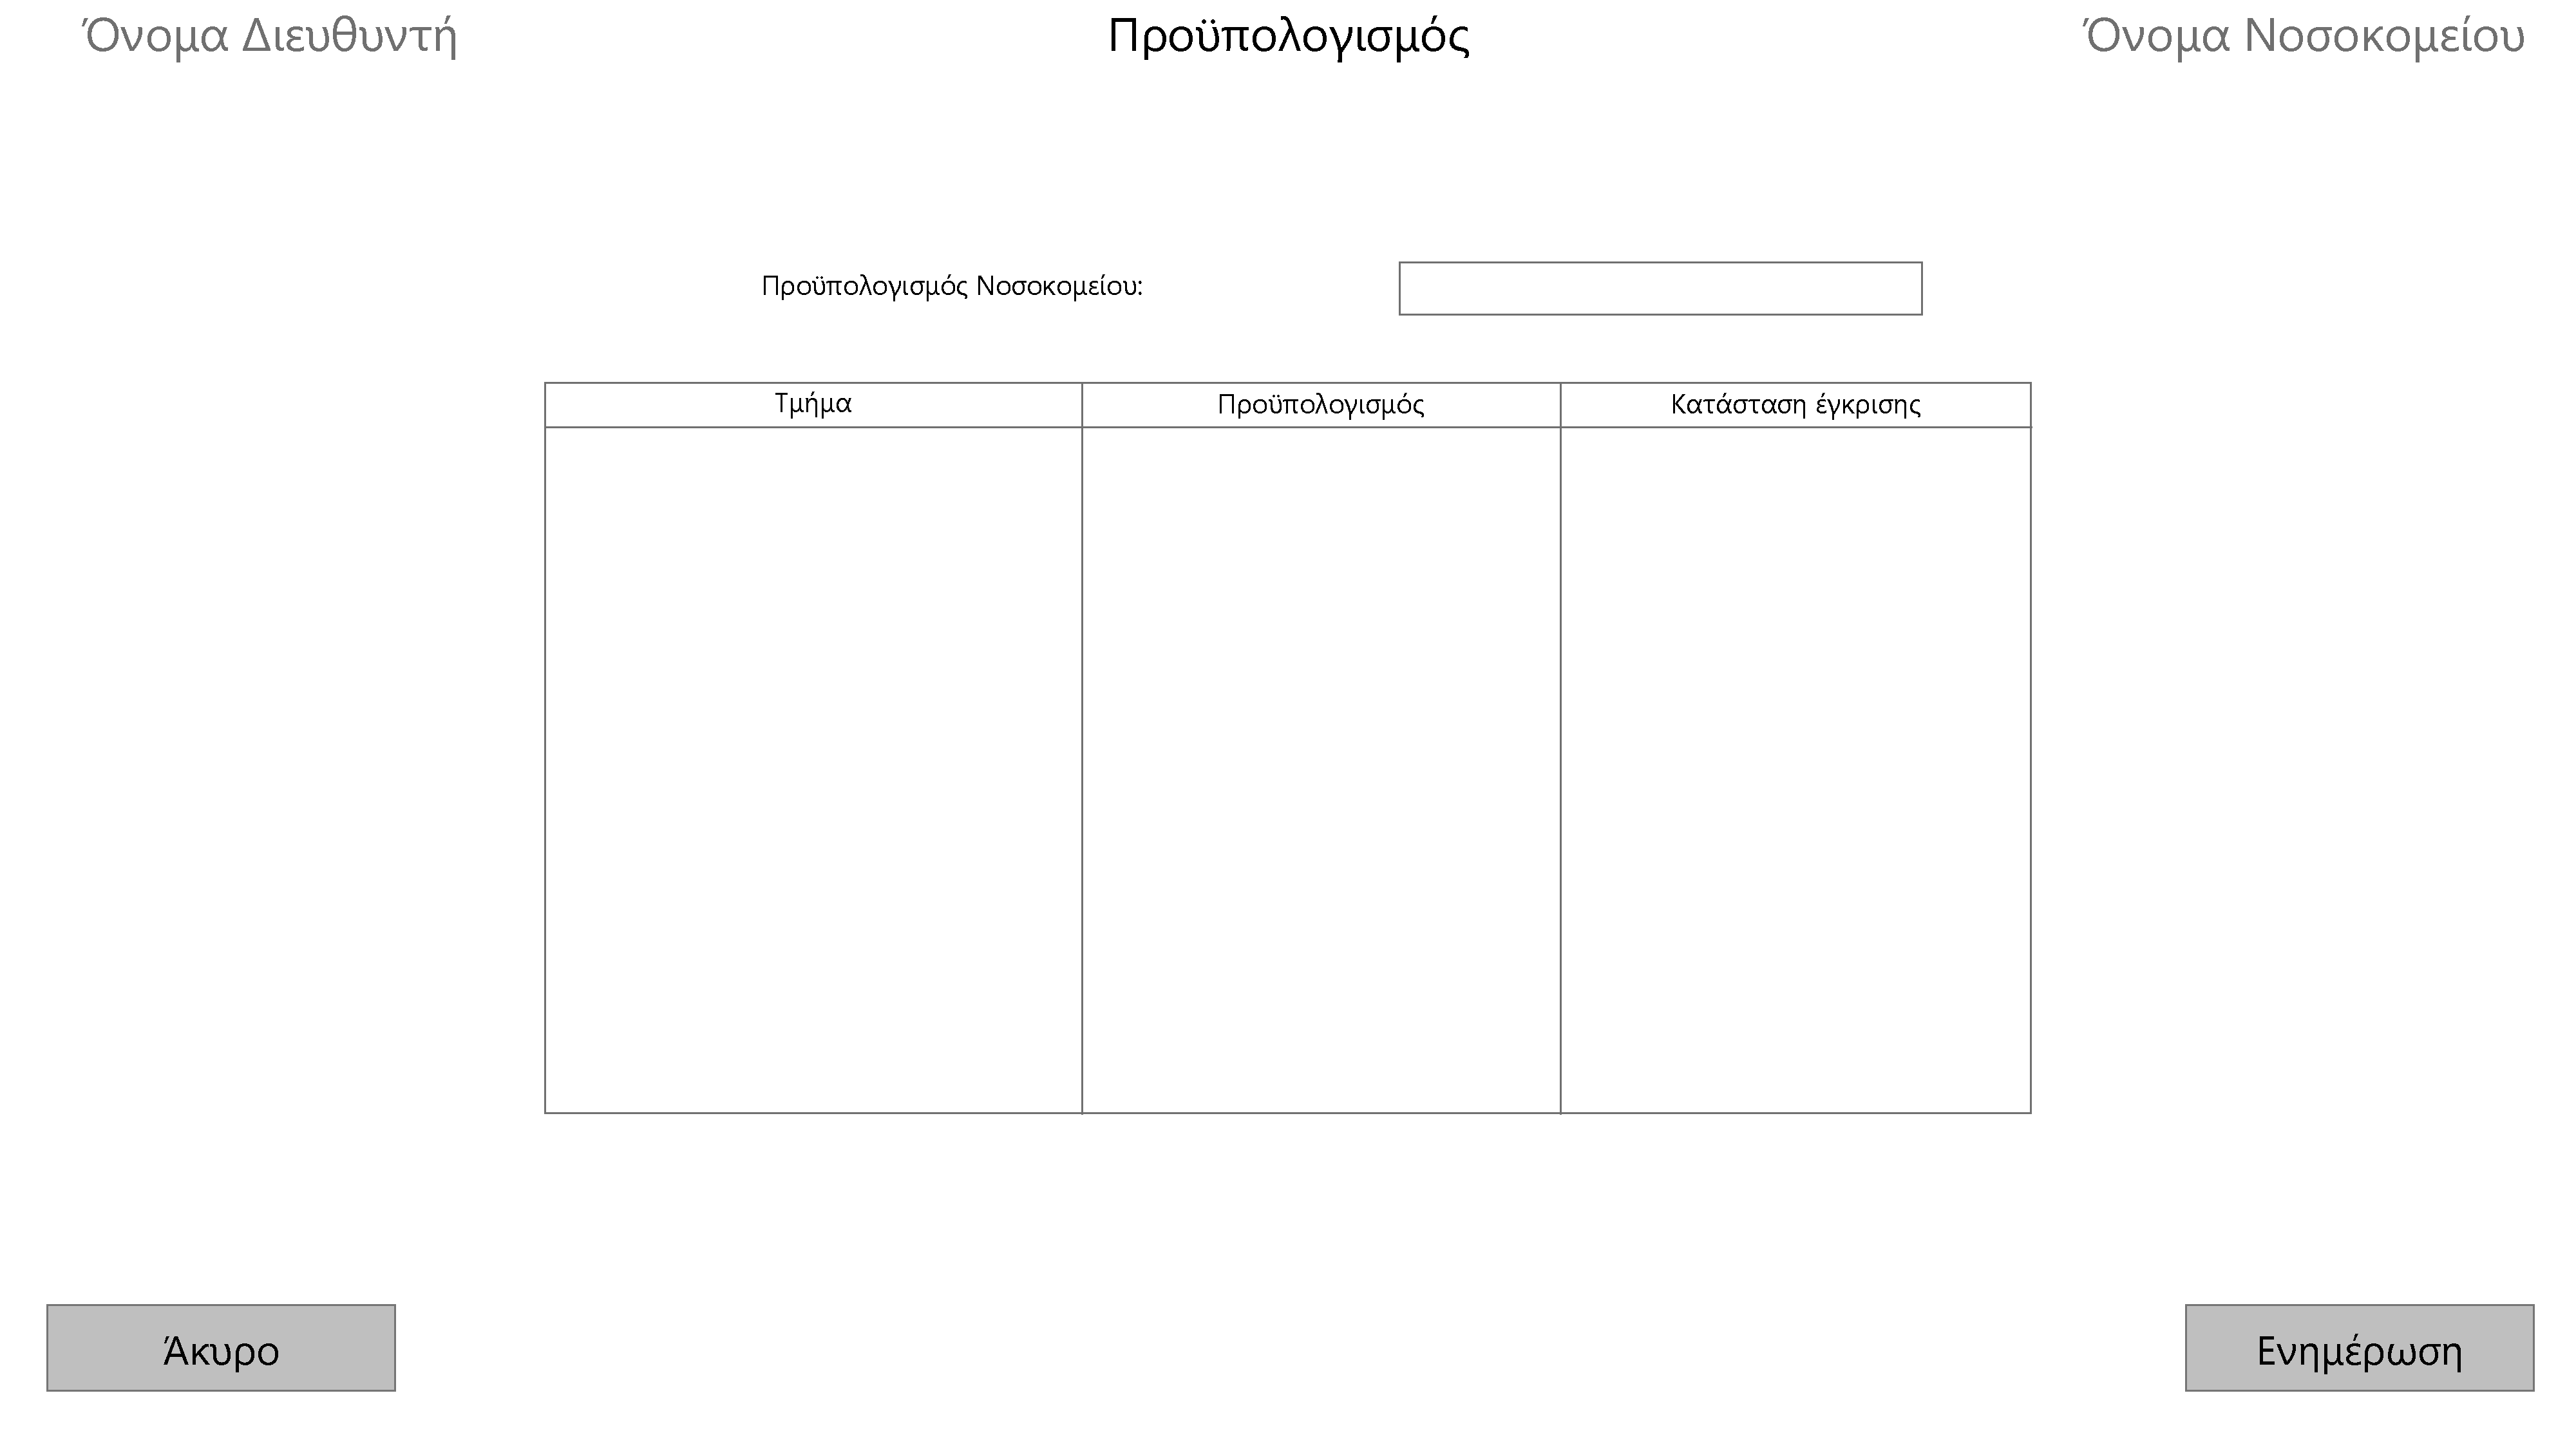
\includegraphics[width=1.1\textwidth]{Διευθυντής Νοσοκομείου Προϋπολογισμός.pdf}
\captionsetup{labelformat=empty}
\caption{Οθόνη 4: Διευθυντής Νοσοκομείου Προϋπολογισμός}
\end{figure}

\begin{figure}[h!]
\centering
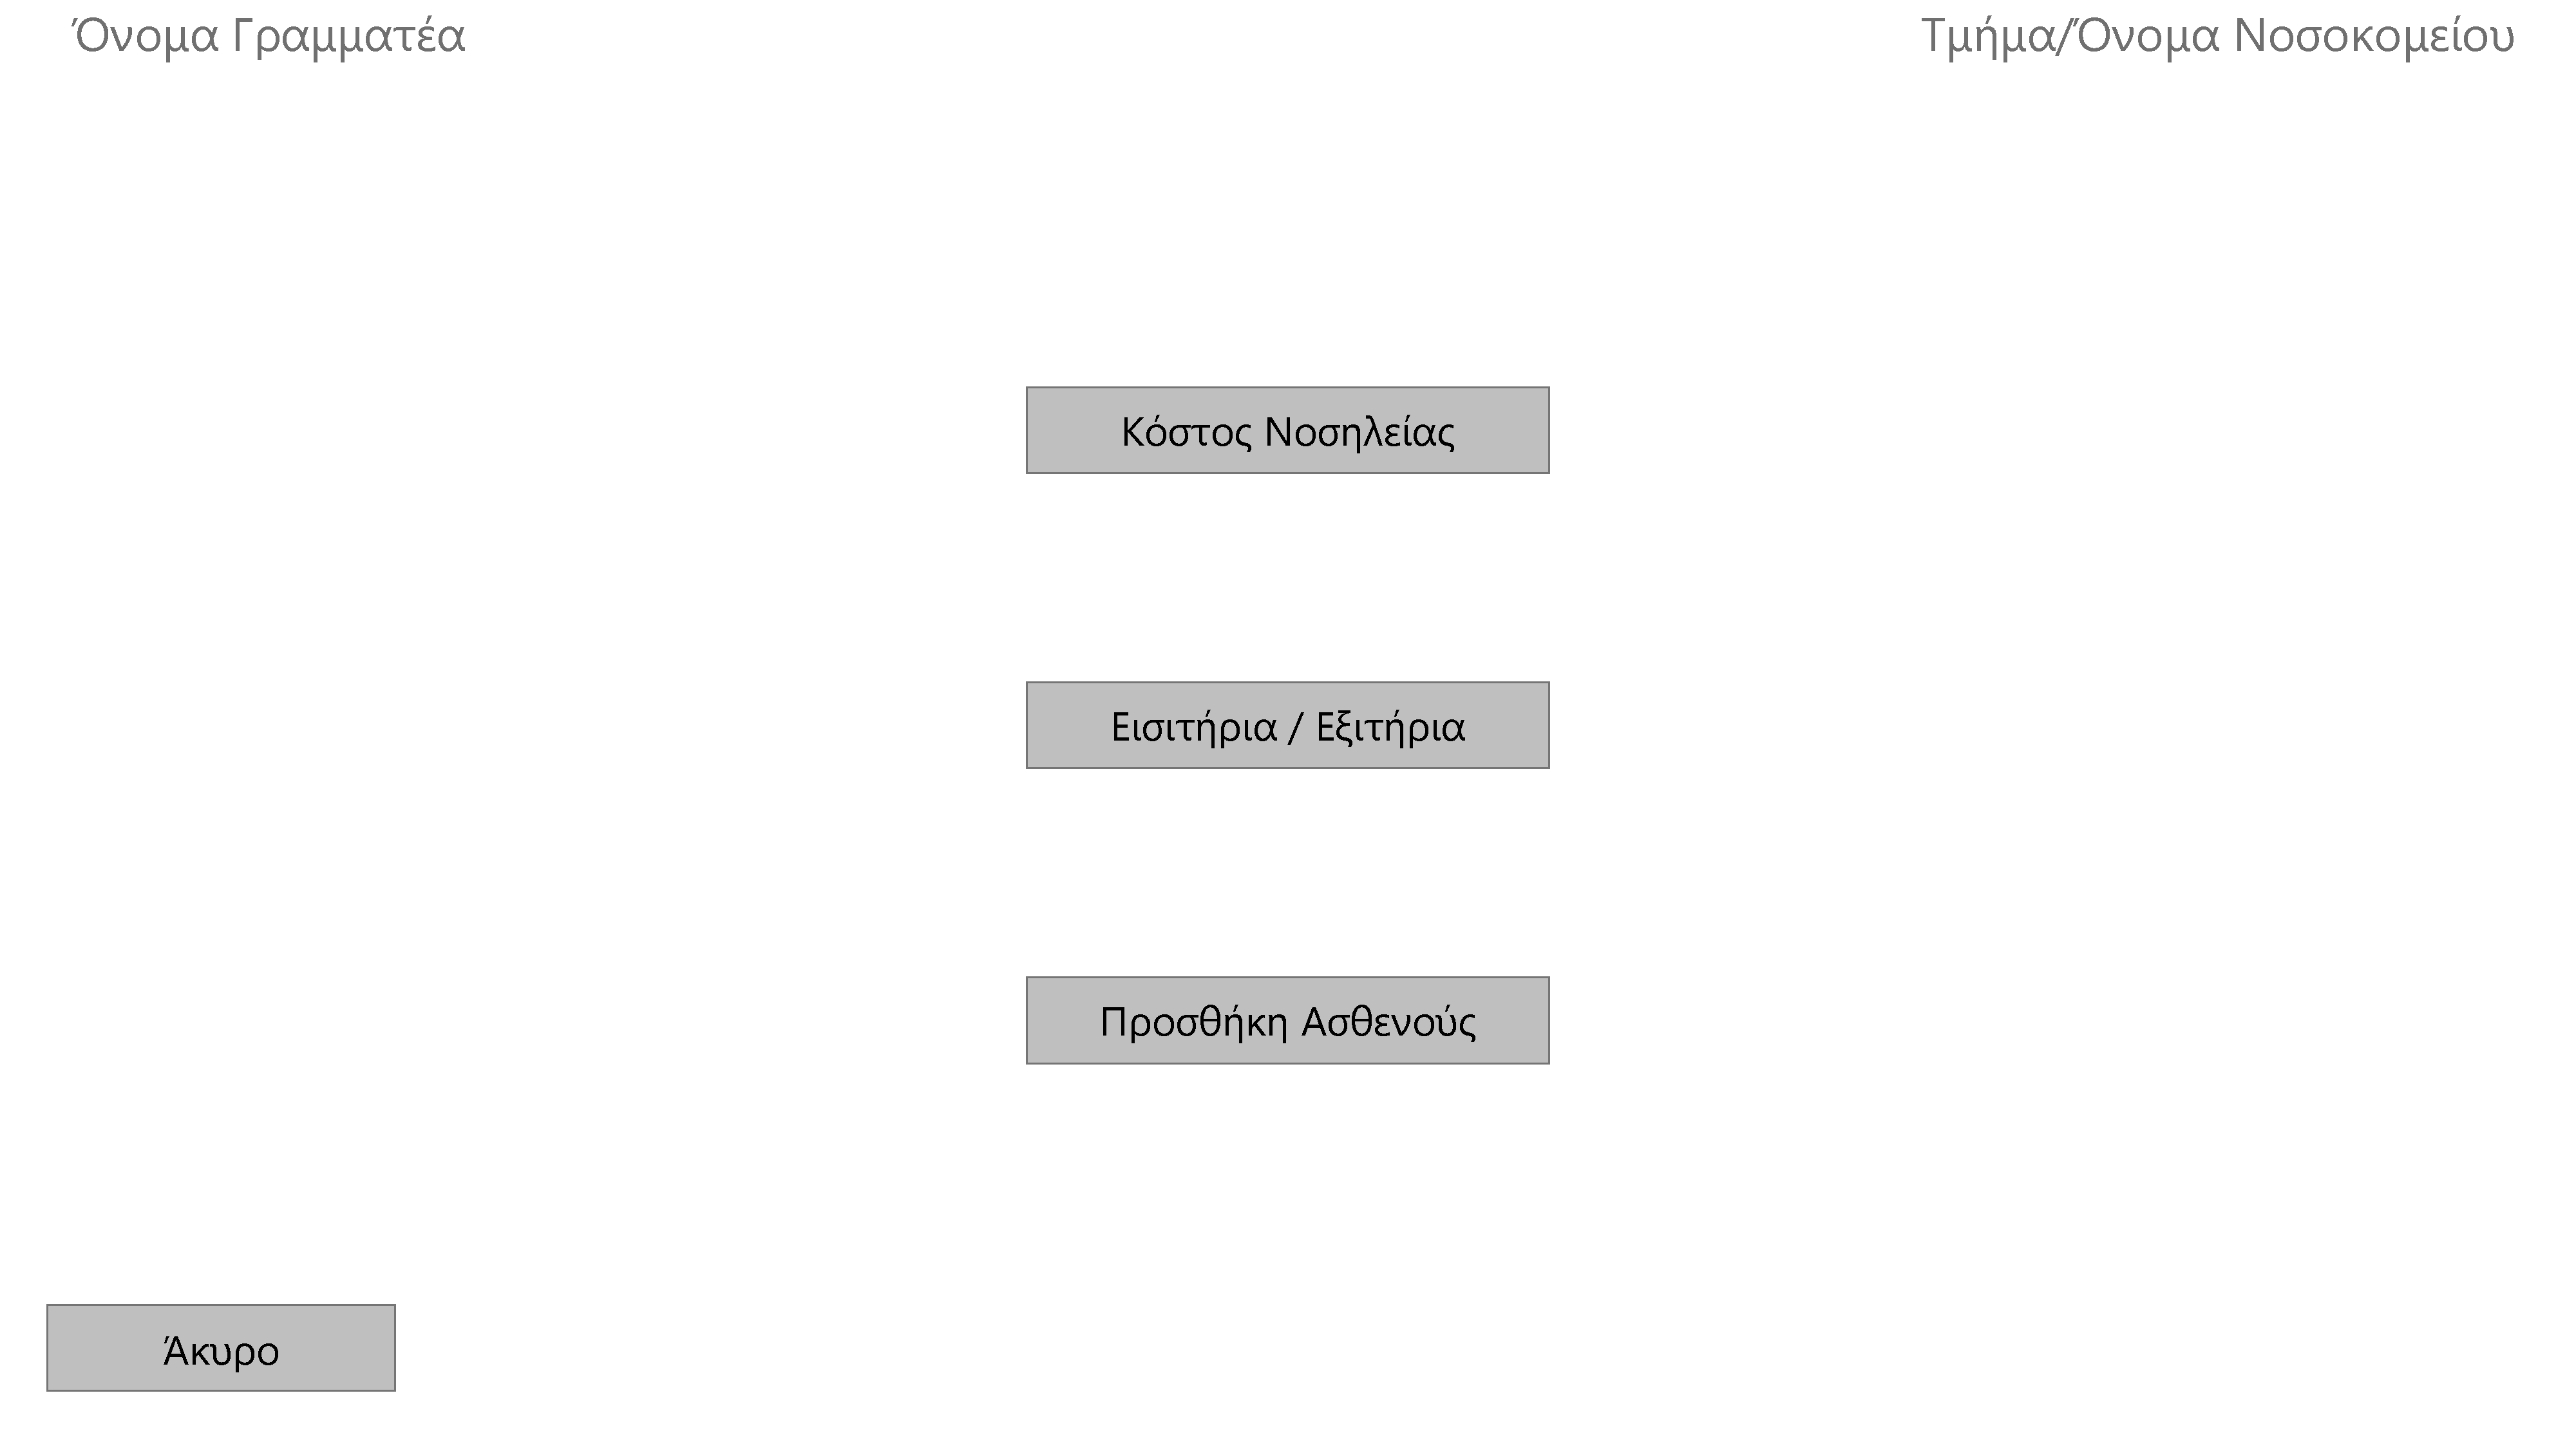
\includegraphics[width=1.1\textwidth]{Γραμματεία Αρχική οθόνη.pdf}
\captionsetup{labelformat=empty}
\caption{Οθόνη 5: Γραμματεία Αρχική οθόνη}
\end{figure}

\begin{figure}[h!]
\centering
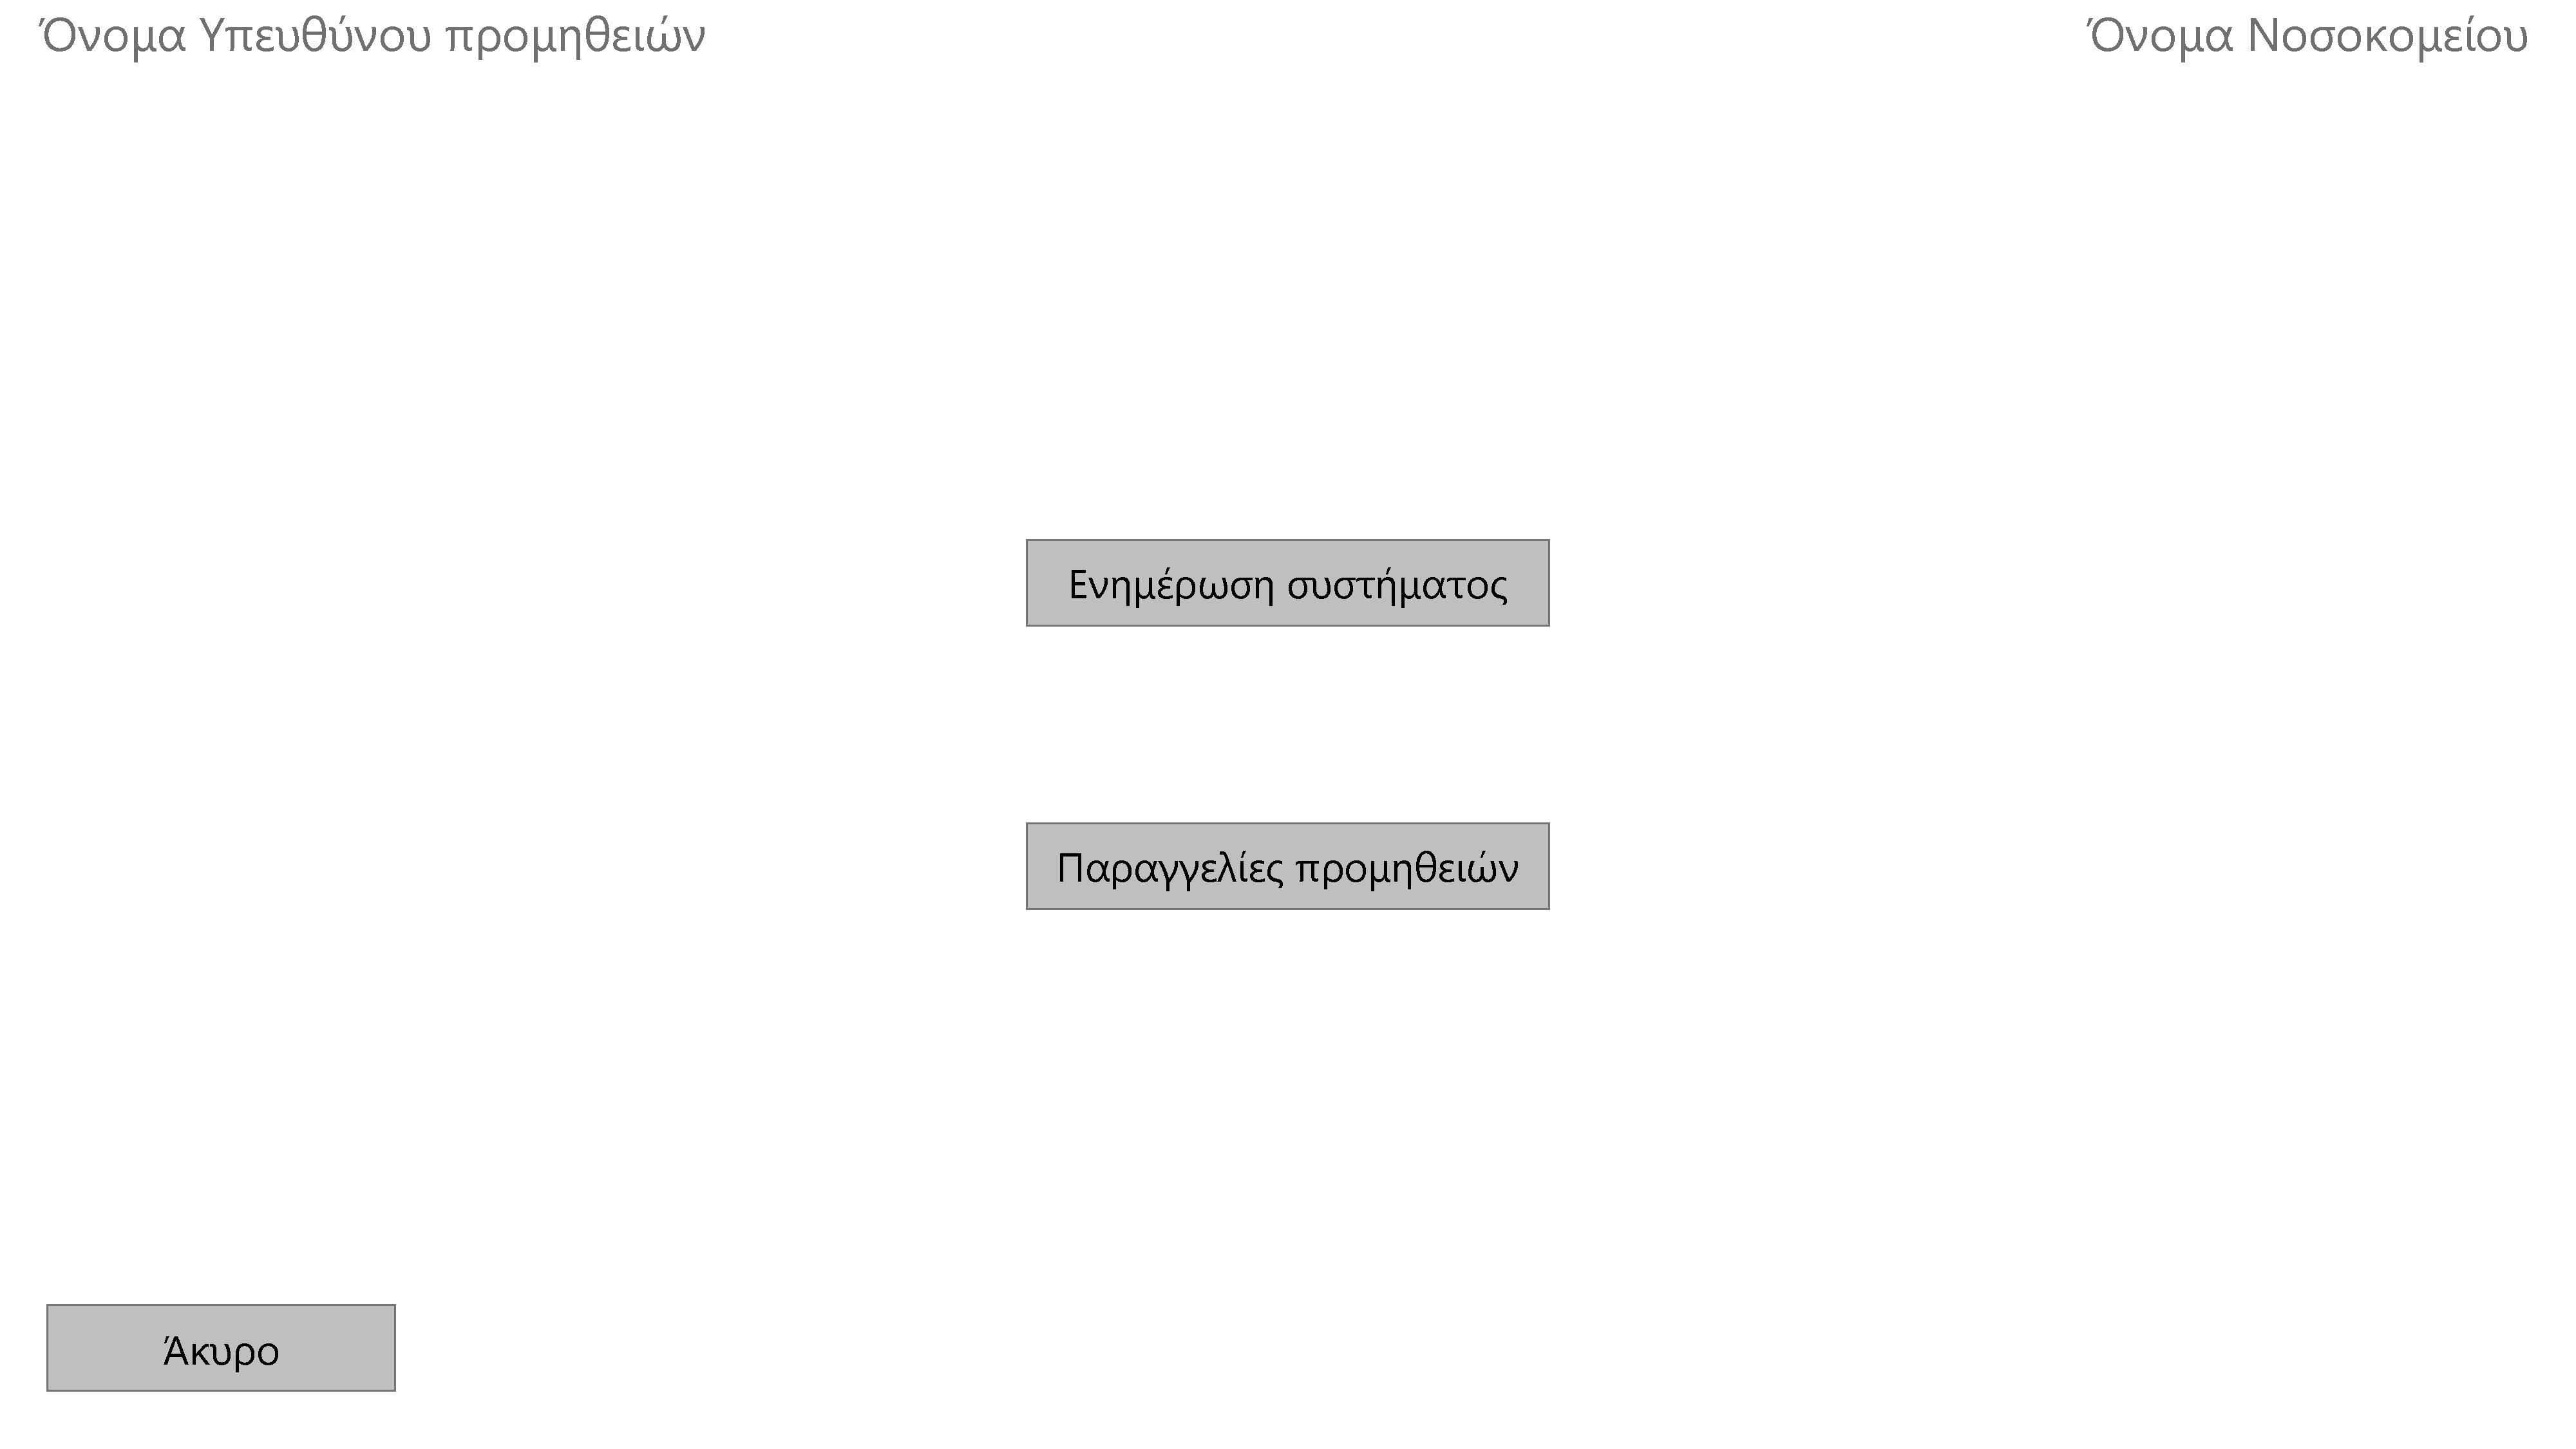
\includegraphics[width=1.1\textwidth]{Υπεύθυνος προμηθειών Αρχική οθόνη.pdf}
\captionsetup{labelformat=empty}
\caption{Οθόνη 6: Υπεύθυνος προμηθειών Αρχική οθόνη}
\end{figure}

%===========================================================
%===========================================================

\bibliographystyle{ieeetr}


\end{document} 
